\documentclass[a4paper, 5p, sort&compress]{elsarticle}%5p for double column
% 
\usepackage{ucs}
\usepackage[utf8x]{inputenc}
\usepackage{amsmath,amssymb,amsfonts,mathtools}
\usepackage[english]{babel}
\usepackage{fontenc}
\usepackage{graphicx}
%\usepackage[caption=false]{subfig}
\usepackage{ulem} 
\usepackage[margin=0pt,font=footnotesize, labelsep=colon]{caption}
\usepackage{tabularx}
\usepackage{multirow}
\usepackage{units}
%\usepackage{subfig}
%\usepackage{siunitx}
\usepackage{booktabs}
\usepackage{bbm}
\usepackage{eurosym}
\usepackage{color}
\usepackage[table]{xcolor}
\usepackage{colortbl}
\usepackage{supertabular}
\usepackage{array,lipsum}
%\usepackage[author-year]{natbib}

\definecolor{rgrey}{gray}{0.75}
\newcommand{\mean}[1]{\langle #1 \rangle}
\newcommand{\E}[0]{\euro \;}
\newcommand{\bs}[1]{\boldsymbol{#1}}
\renewcommand{\rm}{\text }

% Added by emher
\usepackage[noabbrev]{cleveref}
\usepackage[export]{adjustbox}[2011/08/13]
\newcommand{\paren}[1]{\left(#1\right)}
\newcommand{\chromowidth}{1.00 \columnwidth}
\graphicspath{{Figures/}}
\usepackage{algorithm}
\usepackage[noend]{algpseudocode}
\usepackage{placeins}
\usepackage{subcaption}

%\makeatletter
%\def\ps@pprintTitle{%
% \let\@oddhead\@empty
% \let\@evenhead\@empty
% \def\@oddfoot{}%
% \let\@evenfoot\@oddfoot}
%\makeatother
%%%%%%%%%%%%%%%%%%%%%%%%%%%%%%%%%%%%%%
\begin{document}


%*************************************************
\begin{frontmatter}

\title{Optimal heterogeneity of a highly renewable pan-European electricity system}

\author[label1]{Emil H. Eriksen}
\ead{emilhe@phys.au.dk}
%\author[label2]{Benjamin Sairanen}
\author[label2,label3]{Martin Greiner}
\ead{greiner@eng.au.dk}
\address[label1]{Department of Physics and Astronomy, Aarhus University, 8000 Aarhus C,  Denmark}
\address[label2]{Department of Mathematics, Aarhus University, 8000 Aarhus C,  Denmark}
\address[label3]{Department of Engineering, Aarhus University, 8200 Aarhus,  Denmark}


\begin{abstract}
  The resource quality and the temporal production pattern of variable
  renewable energy sources vary significantly across Europe. A
  homogeneous distribution of wind and solar capacities makes
  inefficient use of the resources, resulting in high system costs. A
  heterogeneous distribution of renewable assets maximising the
  overall capacity factor results in smaller investments in renewable
  capacities, but higher costs of transmission. A local search routine
  is used to find optimal distributions of production capacities
  minimising backup, transmission and renewable capacity costs
  simultaneously, resulting in lower costs of electricity.
\end{abstract}

\begin{keyword}
renewable energy system \sep 
levelised cost of electricity \sep
wind power generation \sep
solar power generation 
\end{keyword}

\end{frontmatter}


%*************************************************************************
\section{Introduction}
\label{sec:one}
%*************************************************************************

The ambitious renewable targets set by the European leaders
\cite{eu2050} imply that the renewable penetration will increase
significantly in the years to come. Electrification of transportation
and other sectors will play a major role in the transition
\cite{Williams12,ecf2050}. At present, the leading renewable
technologies are wind, solar PV and hydro, of which only wind and
solar PV have potential for large-scale expansion. For this reason,
only wind and solar PV are modelled explicitly. Since wind and
solar PV are both variable renewable energy resources (VRES), backup
generation is needed if power outages are to be avoided. Backup
generation equals additional system cost and must thus be kept at a
minimum.

The backup requirements depend on the mismatch between load and VRES
generation. Using the degrees of freedom associated with the choice of
VRES assignments, it is possible to smooth out the aggregated temporal
production pattern or even shape it shape it towards the load
pattern. As a result, the mismatch (and thus the backup requirements)
is lowered.  To decrease the dimensionality of the problem, the
renewable assets are often assigned proportional to the mean load of a
country in accordance with a homogeneous wind/solar mixing
factor. This approach is demonstrated in
\cite{Heide2010,Heide2011} where balancing and storage optimal
wind/solar mixes are found.

Further reductions in backup requirements are possible by exchanging
energy between the countries through a transmission network
\cite{rolando2014,sarah}. Other relevant papers on the advantages and
costs of grid extensions are \cite{Schaber, Schaber2}.

% PUT IN 2050 report stuff here?

In a conventional energy system, the siting of production capacities
is not a concern. No geographical areas are preferable, so the power
plants are simply put where the demand is present. For VRES, the
situation is more complicated. The primary reason is the geographical
variation of the VRES
quality. %On average, a solar photovoltaic (PV) installation in
% Spain will be more productive than an equivalent installation in
% Ireland. On the other hand, a wind farm located in Ireland will be
% productive than an equivalent installation in Spain.
The resource quality is quantified through the capacity factor defined as

\begin{equation}
  \label{eq:1}
  \mbox{CF} = \frac{\mbox{Average production}}{\mbox{Rated capacity}} .
\end{equation}

The capacity factor is a number between 0 and 1, where 0 means no
production and 1 means maximum production at all times. Capacity
factors for the European countries for onshore wind, offshore wind and
solar PV are listed in \cref{tab:capacity-factors}. The capacity
factors were calculated using the Renewable Energy Atlas \cite{REA}
(REA). The VRES layout at country level was chosen as a homogeneous
distribution across the 50\% best sites. For wind conversion, a multi
turbine corrected power curve for the Vestas V90 3.0MW turbine was
assumed. For solar conversion, the Scheuten P6-54 solar PV panel
oriented south and tiled from horizontal to a degree equal to the
latitude of installation was applied.

\begin{table*}[t!]
  \caption{Capacity factors $\text{CF}_n^w$, $\text{CF}_n^{\tilde{w}}$ and  $\text{CF}_n^s$ for onshore wind, offshore wind and solar PV for the European countries.}
  \label{tab:capacity-factors}
  \begin{adjustbox}{center}
    \begin{tabular}{lccclccclccc}  \toprule
      & $\text{\textbf{CF}}_n^w$ & $\text{\textbf{CF}}_n^{\tilde{w}}$ & $\text{\textbf{CF}}_n^s$ &  & $\text{\textbf{CF}}_n^w$ &
      $\text{\textbf{CF}}_n^{\tilde{w}}$ & $\text{\textbf{CF}}_n^s$ &  & $\text{\textbf{CF}}_n^w$ & $\text{\textbf{CF}}_n^{\tilde{w}}$ &
      $\text{\textbf{CF}}_n^s$\\ \midrule
      AT & 0.13 & - & 0.16 & DE & 0.20 & 0.44 & 0.14 & NO & 0.25 & 0.36 & 0.13\\
      BE & 0.22 & 0.40 & 0.14 & GB & 0.32 & 0.44 & 0.13 & PL & 0.17 & 0.34 & 0.14\\
      BA & 0.13 & - & 0.18 & GR & 0.14 & 0.34 & 0.19 & PT & 0.18 & 0.20 & 0.20\\
      BG & 0.12 & 0.19 & 0.18 & HU & 0.12 & - & 0.17 & RO & 0.11 & 0.24 & 0.18\\
      HR & 0.17 & 0.23 & 0.18 & IE & 0.35 & 0.38 & 0.11 & RS & 0.09 & - & 0.18\\
      CZ & 0.15 & - & 0.16 & IT & 0.13 & 0.17 & 0.19 & SK & 0.12 & - & 0.16\\
      DK & 0.37 & 0.45 & 0.13 & LV & 0.23 & 0.34 & 0.13 & SI & 0.07 & - & 0.16\\
      EE & 0.26 & 0.32 & 0.13 & LT & 0.20 & 0.32 & 0.13 & ES & 0.15 & 0.21 & 0.20\\
      FI & 0.18 & 0.33 & 0.11 & LU & 0.19 & - & 0.14 & SE & 0.21 & 0.32 & 0.13\\
      FR & 0.20 & 0.34 & 0.17 & NL & 0.27 & 0.43 & 0.13 & CH & 0.13 & - & 0.18\\ \bottomrule
    \end{tabular}
  \end{adjustbox}
\end{table*}

%Wind turbines produce when it is windy, solar
%PV when it is sunny. Backup is thus needed at windless
%nights.

The second reason is the geographical variation of the temporal
production pattern for a given VRES type. This effect is particularly
important for wind since Europe is large compared to the wind
correlation length of $\approx$ 1000 km \cite{Widen2011}. Similar to
the optimal wind/solar mixes found in \cite{Heide2010,Heide2011},
optimal layouts of each VRES in terms of e.g. balancing can be
derived.

With these points in mind, allocating resources proportional to the
mean load of a country in accordance with a homogeneous wind/solar
mixing factor does not seem ideal. In this paper, the effect of
lifting this homogeneous assumption is explored. Different approaches
to cope with the resulting large number of degrees of freedom are
considered ranging from heuristic layouts constructed from resource
quality knowledge to layouts obtained through numerical
optimization. The objective is to find heterogeneous layouts with
properties superior to the homogeneous layouts, in particular a lower
cost of electricity.

%\textcolor{orange}{Two previous papers \cite{Rombauts11,Roques09} have applied
%Optimal Layout Theory to explore heterogeneous distributions of
%wind resources. They have found that there is a significant decrease
%in the overall risk, or standard deviation, when increasing the
%aggregation region, suggesting that there are benefits in establishing
%a transmission network, as also shown by \cite{Rodriguez2013}. In
%\cite{Elliston}, an out-of-the-box genetic algorithm has been applied
%to find the least-cost scenario for a highly renewable electricity
%system in the Australian National Electricity Market (NEM). They found
%that the least cost scenario was that with a penetration of around
%60\% renewables, consisting of around 70\% wind energy.}

% MAYBE MOVE THIS TO SOMEWHERE ELSE?

% The $\beta$ and CF layouts are derived directly from the capacity
% factor. They do not take the temporal production pattern into
% account. By choosing VRES with different temporal patterns, it is
% possible to reduce the backup needs. For homogeneous layouts, the
% dimensionality of the problem is two (one if $\gamma$ is fixed), and the
% optimum is trivially found. In the heterogeneous case, the
% dimensionality of the problem is 2N. For the 30-node network at hand
% 2N = 60 and the optimization no longer trivial. The quest for optimal
% layouts inside the 60 dimensional search space is the topic of
% \cref{sec:cuckoo-search}.

This paper is organised as follows: \Cref{sec:two} discusses the
general modelling of the electricity system, the key metrics and the
construction of heterogeneous layouts. In \cref{sec:results} the
performance of the different layouts and the resulting renewable
penetrations for individual European countries are
discussed. \Cref{sec:sensitivity-analysis} contains an analysis of the
sensitivity of the results to reductions in solar costs and to
expansions in offshore wind capacities. We conclude the paper with a
discussion on the results and an outlook on future research.

%*************************************************************************
\section{Methods}
\label{sec:two}
%*************************************************************************
\subsection{The electricity network}

The European electricity network is modelled using a 30-node model
where each node represents a country. The nodal load is determined
from historical data, while wind and solar production data are
calculated using a combination of weather data and physical
models \cite{REA}. Initially, wind is assumed to be onshore only. For
each node $n$ the generation from VRES,

% -------------------
\begin{equation}
  G^{R}_{n}(t) = G_{n}^{W} + G_{n}^{S},
\end{equation} 
% -------------------

can be expressed through two parameters. The penetration $\gamma$
determines the amount of energy generated relative to the mean load of
the node,

% -------------------
\begin{equation}
  \mean{G^{R}_{n}} = \gamma_{n} \mean{L_{n}} ,
\end{equation} 
% -------------------

while the mixing parameter $\alpha$ fixes the ratio between wind and solar,
%-------------------
\begin{align}
  \mean{G^{W}} &= \mean{G_{n}^{R}} \alpha_{n}  , \\
  \mean{G^{S}} &= \mean{G_{n}^{R}} \paren{1- \alpha_{n}}  .
\end{align} 
%-------------------

The nodal difference between VRES generation and load

%-------------------
\begin{equation}
  \Delta_{n}(t) = G^{R}_{n}(t) - L_{n}(t)
\end{equation}
%-------------------

is called the mismatch. To avoid power outages, the demand must be
matched at all times. Since storage is not considered, any power
deficits must be covered by backup generation. Dispatchable
resources are not modelled explicitly, but are considered a part of
the backup generation. If $\Delta_{n}(t) \geq 0$, excess energy can be
curtailed $C_{n}(t)$, while if $\Delta_{n}(t) < 0$ backup generation
$G^{B}_{n}(t)$ is needed.
% -------------------
\begin{align}
  C_{n}(t) &= + \max \paren{\Delta_{n}(t),0} \\
  G^{B}_{n}(t) &= - \min \phantom{} \paren{\Delta_{n}(t),0} 
\end{align}
% -------------------

Together the two terms form the nodal balancing
$B_{n}(t) = C_{n}(t) - G^{B}_{n}(t)$.  It is possible to lower the
balancing needs by transmission. Nodes with excess production export
energy $E_{n}(t)$, allowing nodes with an energy deficit to import
energy $I_{n}(t)$ to (partly) cover their energy deficit. The nodal
injection, $E_{n}(t) - I_{n}(t)$, is denoted $P_{n}(t)$. This leads to
the nodal balancing equation,

% -------------------
\begin{equation}
  \label{eq:nodal-balancing}
  G^{R}_{n}(t) - L_{n}(t) = B_{n}(t) + P_{n}(t) .
\end{equation}
% -------------------

The vector of nodal injections $\mathbf{P}$ is called the injection
pattern. The actual imports and exports, and thus the injection
pattern, depend on the business rules of the nodal interactions. It is
convenient to express business rules in terms of a two step
optimization problem. The top priority is to minimize the backup
generation,

% -------------------
\begin{equation}
  \label{eq:step1}
  \begin{aligned}
    \text{Step 1: \hspace{15pt}}& \underset{\mathbf{P}, \mathbf{F}}{\text{min}}
    & & \sum_{n} \frac{\paren{G_{n}^{B}}^{2}}{L_{n}} \\
    & \text{s.t.}
    & & \sum_{n} P_{n} = 0 \\ %F_{l}^{-} \leq F_{l} \leq F_{l}^{+}
    & \text{s.t.}
    & & F_{l}^{-} \leq F_{l} \leq F_{l}^{+}
  \end{aligned}
\end{equation}
% -------------------

where $F_{l}$ is the flow in link $l$ and $F_{l}^{\pm}$ denote any
flow constraints. While \cref{eq:step1} fixes \textbf{P}, the problem
remains degenerate in \textbf{F}. As an example, if \textbf{F'} is a
solution, any solution \textbf{F''} obtained by adding a circular flow
to \textbf{F'} will also be a solution. The degeneracy is removed by a
second optimization step. To ensure that \textbf{F} resembles a
physical flow, the objective is chosen as minimization of the sum of
squared flows \cite{Magnus}.

% -------------------
\begin{equation}
  \begin{aligned}
    \label{eq:step2}
    \text{Step 2: \hspace{15pt}} & \underset{\mathbf{F}}{\text{min}}
    & & \sum_{l} F_{l}^{2} \\
    & \text{s.t.}
    & & \mathbf{P} = \mathbf{P}^{*} \\ %F_{l}^{-} \leq F_{l} \leq F_{l}^{+}
    & \text{s.t.}
    & & F_{l}^{-} \leq F_{l} \leq F_{l}^{+} \\
    %& \text{s.t.}
    %& & G_{n}^{B} = G_{n}^{B*} ,
  \end{aligned}
\end{equation}
% -------------------

where $\mathbf{P}^{*}$ is the injection pattern found in step 1.

%\footnote{This is only strictly true for unconstained
  %flow. However, even when flow constraints are present, the minimal
  %flow solution represents a fairly good approximation\cite{Magnus}.}.

\subsection{Key metrics}

Inspired by \cite{Sensitivity}, the energy system cost is calculated
based on a few key parameters. Besides the cost of the VRES
capacities, $\mathcal{K^{W}}$ and $\mathcal{K^S}$, costs for the
backup system and the transmission network are included. The backup
system cost is split into two components, the cost of backup capacity
$\mathcal{K}^{B}$ (including maintance) and the cost of backup energy
$E^{B}$. The backup capacity cost covers expenses related to
construction and to keeping the power plants online while the backup
energy cost accounts for actual fuel costs. Expressed in units of
the average yearly load, the backup energy is given by

% -------------------
\begin{equation}
  \label{eq:backup-energy}
  E^{B} =\frac{\sum_{n} \sum_{t} G^{B}_{n}(t)}{\sum_{n} \sum_{t}
    L_{n}(t)} = \sum_{n} \frac{\langle G^{B}_{n} \rangle}{\langle L_{n}
    \rangle} .
\end{equation}
% -------------------

In principle, the backup capacity is fixed by a single extreme
event. However with this definition, the results will be highly
coupled to the particular data set used. To decrease the coupling, the
99\% quantile is used rather than the maximum value,

\begin{equation}
  \label{eq:2}
  q_{n} = \int _{0} ^{K_{n}^{B}} p_{n}(B_{n})dB_{n},
\end{equation}

where $p_{n}(B_{n})$ is the time sampled distribution of backup power
and $q_{n} = 0.99$. With this choice, the backup system will be able
to cover the demand 99\% of the time. The remaining 1\% is assumed to
be covered by unmodelled balancing initiatives, e.g. demand side
management. Given the nodal values $\mathcal{K}^{B}$ is calculated by
summation,

\begin{equation}
  \label{eq:4}
  \mathcal{K}^{B} = \sum_{n} \mathcal{K}^{B}_{n} .
\end{equation}

In accordance, the transmission capacity $\mathcal{K}^{T}$ is defined
so that the demand is met 99\% of the time. Transmission can be
positive and negative, but since links are assumed bidirectional, only
the magnitude (not the sign) of the flow is to be considered. Hence

\begin{equation}
  \label{eq:2}
  q_{n} = \int _{0} ^{K_{n}^{T}} p_{l}(|F_{l}|)dB_{n},
\end{equation}

where $p_{l}(|F_{l}|)$ is the time sampled distribution of absolute
flows and $q_{n} = 0.99$. Since the link length varies,
$\mathcal{K}^{T}$ is not calculated directly by summation, but instead
as a weighted sum,

\begin{equation}
  \label{eq:4}
  \mathcal{K}^{T} = \sum_{l} \mathcal{K}^{T}_{l} L_{l},
\end{equation}

where $L_{l}$ denotes the length of link $l$.

% -------------------

\subsection{Cost modelling}
\label{sec:cost-modelling}

Cost assumptions for the elements of an energy system vary greatly
across the literature \cite{Sensitivity}. In this study, cost
assumption published by \cite{Rolando} have been adapted with a single
modification. The cost of solar has been reduced by 50\% in accordance
with near future solar PV panel price projections \cite{irena}. The
resulting estimates are listed in \cref{tab:cost-assumptions}. In
general, the cost assumptions are in the low end for VRES which
reflects the expectation that the cost of VRES will go down in the
future as the penetration increases \cite{Fraunhofer}.

\begin{table}[h!]
  \centering
  \caption{Cost assumptions for different assets.}
  \label{tab:cost-assumptions}
  \begin{tabular}{lrrr}  \toprule
    Asset & CapEx & Fixed OpEx & Variable OpEx\\
    & [€/W] & [€/kW/y] & [€/MWh]\\ \midrule
    CCGT & 0.90 & 4.5 & 56.0\\
    Solar PV & 0.75 & 8.5 & 0.0\\
    Offshore wind & 2.00 & 55.0 & 0.0\\
    Onshore wind & 1.00 & 15.0 & 0.0\\
    \bottomrule
  \end{tabular}
\end{table}

From the VRES penetration, the mixing factor and the mean load, the
effective production of each node can be calculated. Dividing by the
associated capacity factor, the capacity is obtained. Except for
transmission capacity, the present value of each element can be
calculated directly as

% -------------------
\begin{equation}
  \label{eq:6}
  V = \text{CapEx} + \sum_{t} \frac{\text{OpEx}_{t}}{\paren{1 + r}^{t}}
\end{equation}
% -------------------

where $r$ is the return rate assumed to be 4\%. The transmission
capacity cannot be translated directly into cost as the cost depends
on the length and the type of the link. Link lengths have been
estimated as the distance between the country capitals. Link costs are
assumed to be 400\euro{}
per km for AC links and 1,500\euro{}
per km for HVDC links. For HVDC links, an additional cost of
150,000\euro{}
per converter station (one in each end) is
added \cite{McKinsey, Schaber, Schaber2}. The layout of AC and
DC links has been constructed by \cite{rolando2014} from ENTSO-E data.

%The layout of AC and DC lines
%was determined according to the existing European network reported by
%ENTSO-E for the year 2011 \cite{ENTSOEcaps} and new predicted lines
%until 2014 \cite{NorNed, BritNed}.

Given the element costs, the system cost $V_{sys}$ is calculated by
summation. To allow for comparison of different energy systems, the
levelised cost of electricity (LCOE) is a convenient measure. The LCOE
is the cost that every unit of energy produced during the lifetime of
the project must have to match the present value of
investment \cite{Short1995},

\begin{equation}
  \label{eq:7}
  \text{LCOE} = \frac{V_{sys}}{\sum_{t} \frac{L_{EU,
        t}}{\paren{1+r}^{t}}} .
\end{equation}

Life times of 25 years for solar PV and onshore wind, 20 years for
offshore wind, 30 years for CCGT plants and 40 years for transmission
infrastructure were assumed. See \cite{Sensitivity} for more details
on the cost calculation.

Because extreme events in terms of backup capacity (all countries have
a large energy deficit) and transmission capacity (some countries have
a energy deficit while others have excess production) are generally
not overlapping, scaling down $\mathcal{K}^{T}$ with some fraction
$\beta$ tends to lowert the LCOE since $\mathcal{K}^{B}$ is not increased
accordingly. This point is illustrated in
\cref{fig:transmission-lcoe}.

\begin{figure}[h!]
  \centering
  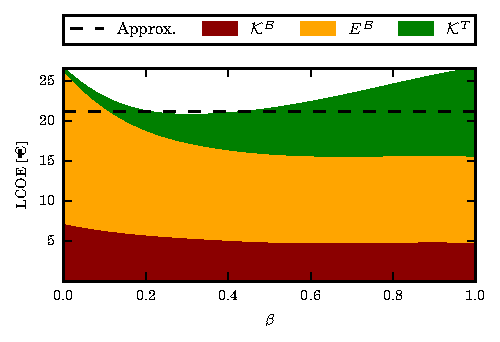
\includegraphics[width = \columnwidth]{constrainedSync}
  \caption{Non VRES LCOE components for different values of $\beta$. The
    dotted line indicates the approximated LCOE (see text).}
  \label{fig:transmission-lcoe}
\end{figure}

\Cref{fig:transmission-lcoe} reveals that the LCOE values at
$\beta = 1$ and $\beta = 0$ are practically equal. However, in the
intermediate region a significant drop in the LCOE is observed. The
optimal value of $\beta$ depends of the electricity system being analysed
and on the specific LCOE definition. Obtaining the lowest possible
LCOE would thus require system individual
optimization. To avoid the additional complexity associated with a
such optimization and to to define the LCOE function in a consistent
way, the LCOE will consistently be calculated using the synchronized
export scheme at $\beta=1$, but with only 50\% of the
$\mathcal{K}^{T}$ cost. The approximation is shown as a dotted line in
\cref{fig:transmission-lcoe}. While the approximation is not perfect,
the inaccuracy associated with the approximation is negligible
compared to the uncertainty of the cost estimates.

\subsection{Heuristic layouts}
\label{sec:heuristic-layouts}

The simplest way to distribute the renewable resources would be to
assign the resources homogeneously (relative to the mean load of the
node) so that $\gamma_{n} = \gamma$ (and $\alpha_{n} = \alpha$). However this assignment
might not be ideal since the capacity factors vary significantly
between the nodes. Having this point in mind, an intuitive way to
proceed would be to assign resources proportional to $\nu$. To
generalise the idea, $\nu$ is raised to an exponent $\beta$ as suggested by
\cite{Rolando}. For a wind only layout, the nodal $\gamma$ values are given by

\begin{equation}
  \label{eq:8}
  \gamma_{n}^{W} = \gamma \paren{\nu^{W}_{n}}^{\beta} \frac{\langle L_{EU}
    \rangle}{\sum_{m} \langle L_{m}
    \rangle \paren{\nu^{W}_{m}}^{\beta}}
\end{equation}

where $\gamma$ is the overall penetration assumed to be 1. An equivalent
expression for the solar only layout is obtained by the substitution
$W \to S$. Examples for $\beta$ = 1 are shown in \cref{fig:examples}. In
the layout illustrations, each bar represents a country $n$. The
height of the bar is $\gamma_{n}$ while the mix $\alpha_{n}$ between onshore
wind (dark blue) and solar (yellow) is expressed through the bar
colouring. $\beta$ layouts for any value of $\alpha$ can be constructed as a
linear combination of the wind and solar only layouts with

% For $\alpha = 1$, the beta layout vector
% $\boldsymbol x _{\beta}(\alpha = 1)$ is defined by \cref{eq:8} and along with
% the trivial identity $\alpha_{n} = 1$

\begin{equation}
  \label{eq:9}
  \gamma_{n} = \alpha \gamma^{W}_{n} + (1-\alpha) \gamma^{S}_{n} 
\end{equation}

and

\begin{equation}
  \label{eq:9}
  \alpha_{n} = \frac{\alpha \gamma_{n}^{W}}{\alpha \gamma_{n}^{W} + (1-\alpha) \gamma_{n}^{S}} .
\end{equation}

% The transformation of $\alpha$ in \cref{eq:9} decouples the assignment of
% wind and solar PV. 

For practical reasons, it is not possible to realise arbitrarily
heterogeneous layouts. To constrain heterogeneity, the heterogeneity
factor K is introduced by requiring

\begin{equation}
  \label{eq:k-factor}
  \frac{1}{\text{K}} \leq \gamma_{n} \leq \text{K} .
\end{equation}

With this definition, K = 1 corresponds to a homogeneous layout while
K = $\infty$ represents unconstrained heterogeneity.

Although the capacity factor of a $\beta$ layout is higher than the
capacity factor of the homogeneous layout (for $\beta$ $>$ 0), it is
possible to achieve an even higher capacity factor without violating
the constraints in \cref{eq:k-factor}. In the wind/solar PV only
cases, the capacity factor is maximised by assigning $\gamma_{n}$ = K to
the countries with the highest capacity factor for wind/solar PV and
$\gamma_{n} = \frac{1}{\text{K}}$ to the remaining countries, except for a
single in-between country. Examples for K = 2 are shown in
\cref{fig:examples}. Similar to the $\beta$ layouts, CF layouts for
arbitrary $\alpha$ values can be constructed as linear combinations of the
wind and solar PV only layouts.

\begin{figure*}[h!]
  \centering
  \begin{subfigure}{2\columnwidth}
    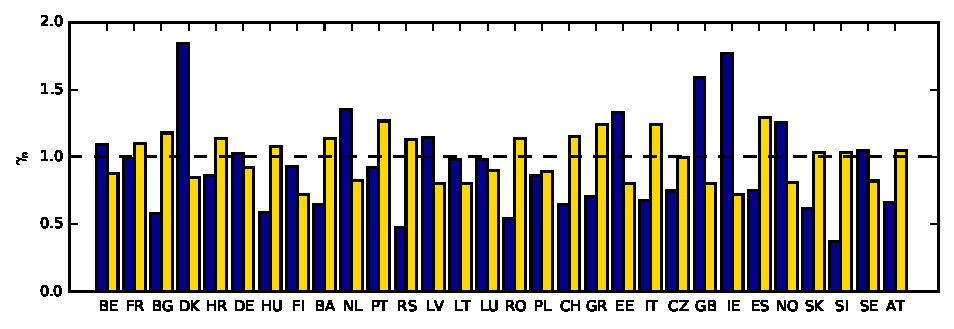
\includegraphics[width = \chromowidth, center]{beta=1}
    \caption{Examples of $\beta$ layouts for $\beta = 1$.}
    \label{fig:betaExamples}    
  \end{subfigure}
  \begin{subfigure}{2\columnwidth}
    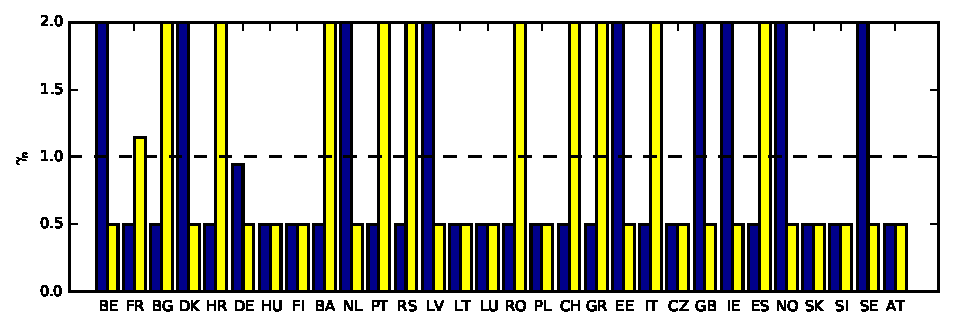
\includegraphics[width = \chromowidth, center]{k=2cfMax}
    \caption{Examples of CF layouts constrained by K = 2 .}
    \label{fig:cfMaxExamples}    
  \end{subfigure}
  \caption{Examples of heuristic layouts. In each sub figure, two sets
    of bars corresponding to the $\alpha = 1$ and the $\alpha = 0$ layouts are
    shown.}
  \label{fig:examples}
\end{figure*}

\subsection{Optimized layouts}
\label{sec:optimized-layouts}

The optimization objective is minimization of the LCOE with respect to
the 60 variables
$\gamma_{1}, ..., \gamma_{N}, \alpha_{1}, ..., \alpha_{N}$.  A number of optimization
algorithms were tested of which a custom local search algorithm
implementation denoted Greedy Axial Search
(GAS) %described in \cref{sec:cuckoo-search},
was found to be most effective. All optimized layouts have been
obtained using the GAS routine. These layouts will be denoted GAS
layouts.

\FloatBarrier

\section{Results}
\label{sec:results}

An overview of the key variables is shown in \cref{fig:overview}. For
backup energy and backup capacity, the optimal $\alpha$ value is around
0.9, which is slightly higher than the values found by
\cite{Heide2010,Heide2011}. The difference can be attributed to the
different data sets used for wind and solar PV. For transmission
capacity, the curves are quite similar for the $\beta$ layouts with a
minimum around $\alpha = 0.5$. For the CF layouts a larger increase in
$\mathcal{K}^{T}$ is observed as K is incremented. This observation is
in qualitative agreement with intuition since the CF layouts are
generally more extreme than the $\beta$ layouts (see
e.g. \cref{fig:optLayouts}).

%, indicating a high share of
%solar PV. While the wind correlation length is around $\approx$ 1000
%km \cite{Widen2011} and thus smaller than Europe, the occurrence of
%sun light is highly correlated for the European countries.
%\cite{Timo}. 
%Therefore, a high wind share causes more power to flow
%between the countries.

The main variable of interest, the LCOE, has a maximum at $\alpha = 0$. It
drops steadily as $\alpha$ is increased until around
$\alpha = 0.8$ where the minimum is located. The high cost at
$\alpha = 0$ is caused by a combination of high backup energy/capacity
costs and the fact that the CF of solar is generally lower than for
onshore wind. The cost of producing one unit of energy is thus higher for
solar than for onshore wind even though the CapEx is lower for solar.

\begin{figure*}[p]
  \centering
  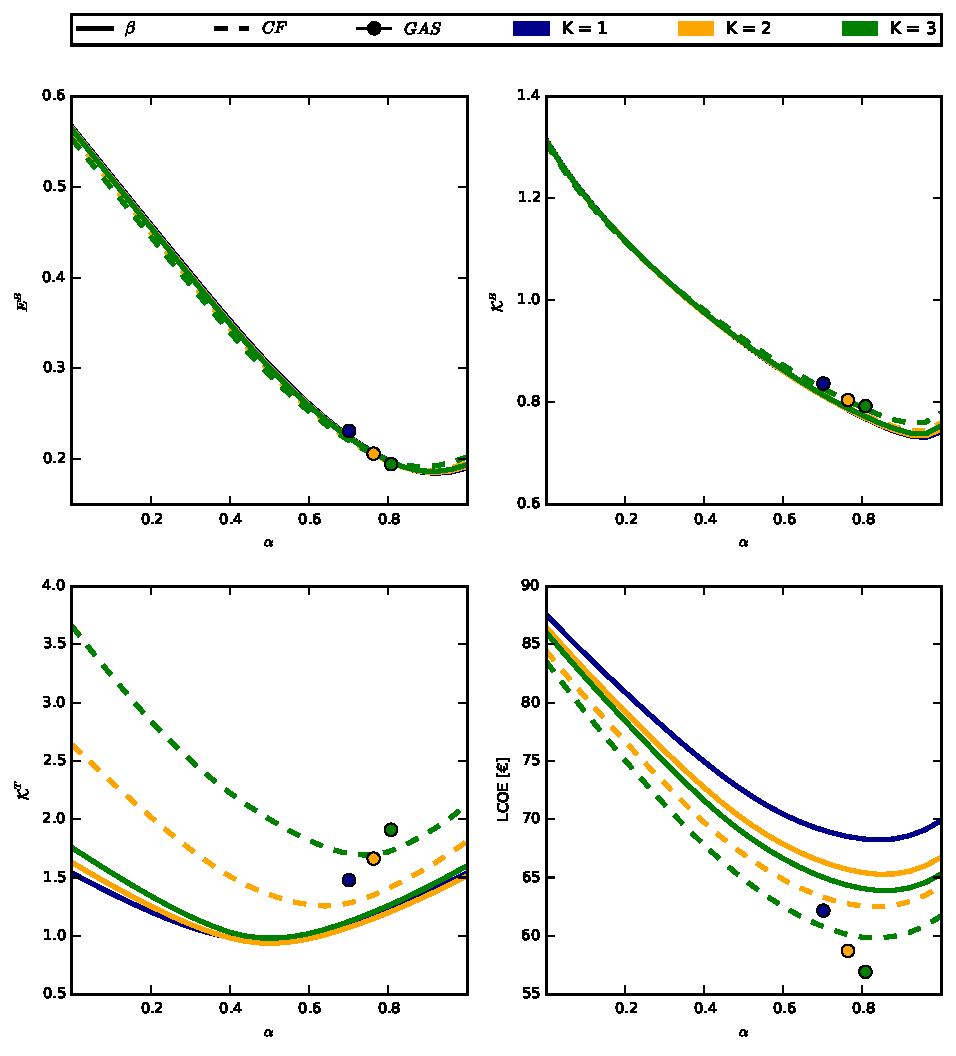
\includegraphics[width = 2 \columnwidth]{dataSync}
  \caption{Overview of the key variables and the associated LCOE as a
    function of $\alpha$ for the $\beta$ (solid line) and CF (dotted
    line) layouts. The GAS layouts are plotted as dots. Heterogeneity
    factors of K = 1 (blue), K = 2 (yellow) and K = 3 (green) are
    shown.}
  \label{fig:overview}
\end{figure*}

The component wise costs for the optimal $\beta$, CF and GAS layouts
are shown in \cref{fig:cost}. From this figure it is clear that the
VRES cost is dominating. Compared to the $\beta$ and CF layouts, the
GAS layouts include a slightly larger solar component. The
magnitude of the solar component for the GAS layouts drops with
increasing K value. As the heterogeneity constraints are loosened wind
becomes more favourable since it becomes possible to allocate more
resources to the sites with a very high CF. A similar effect is
present for solar, but it is less dominant since the best CF for solar
(0.20, Spain) is much smaller than for wind (0.37 for Denmark).

\begin{figure}[h!]
  \centering
  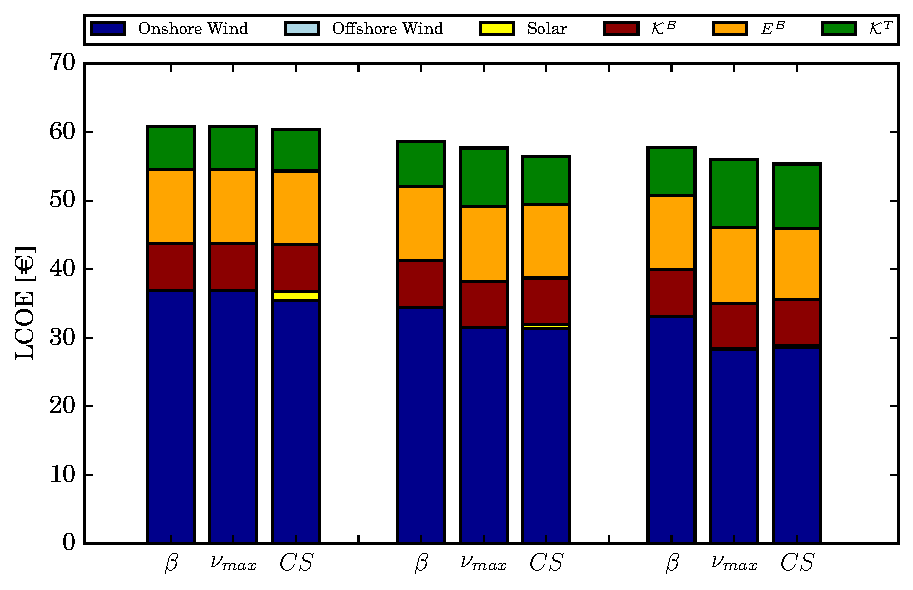
\includegraphics[width = \columnwidth]{costVE50}
  \caption{Component wise LCOE for the optimal $\beta$, CF and GAS layouts
    for K = 1 (left), 2 (middle) and 3 (right).}
  \label{fig:cost}
\end{figure}

The optimal $\beta$, CF and GAS layouts are shown in
\cref{fig:optLayouts}. Note that for $K=1$, the $\beta$ and the
CF layouts are both equal to the homogeneous layout. From
\cref{fig:cfMaxOpt,fig:agdOpt} we see that the CF and the GAS
layouts are quite similar. These figures also explain why the GAS
routine is able to include a solar component at a competitive cost;
unlike the $\beta$ and CF layout definitions, the GAS routine has
the freedom to assign solar only to countries with poor wind
resources, e.g. Serbia (RS) and Slovenia (SI). % In addition, the GAS
%routine reallocates some of the wind resources%, e.g. from Latvia (LV)
%to Portugal (PT), 
%to counteract power flows, see \cref{fig:links}.

%The $\beta$ layouts are shown in \cref{fig:betaOpt} and the CF layouts in \cref{fig:cfMaxOpt}. In
%both cases, $\alpha = 1$ correspond to the cost optimal mix. The optimal
%$GAS$ layouts are shown in \cref{fig:agdOpt}.

\begin{figure*}[p]
  \centering
  \begin{subfigure}{2\columnwidth}
    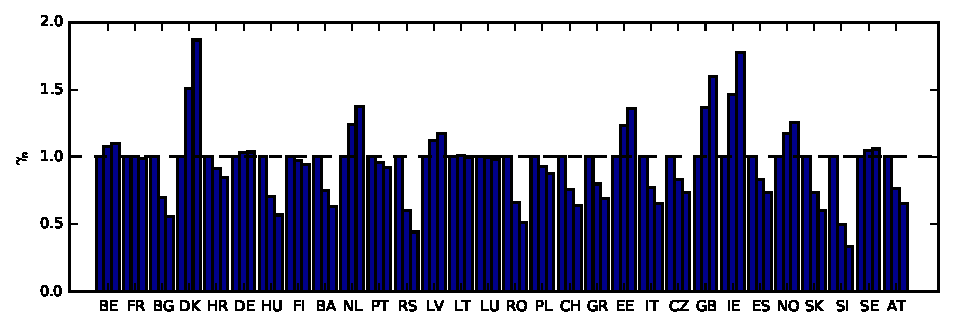
\includegraphics[width = \chromowidth, center]{betaLayouts}
    \caption{Optimal $\beta$ layouts (optimal mix at $\alpha = 0.84$).}
    \label{fig:betaOpt}    
  \end{subfigure}
  \begin{subfigure}{2\columnwidth}
    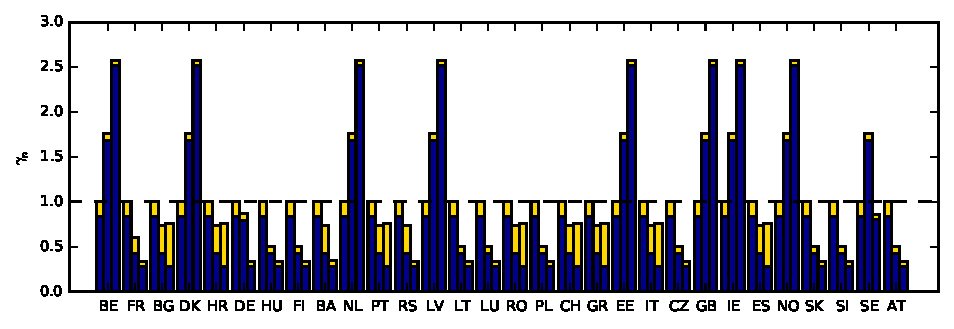
\includegraphics[width = \chromowidth, center]{cfMaxLayouts}
    \caption{Optimal CF layouts (optimal mix at $\alpha = 0.84$).}
    \label{fig:cfMaxOpt}    
  \end{subfigure}
  \begin{subfigure}{2\columnwidth}
    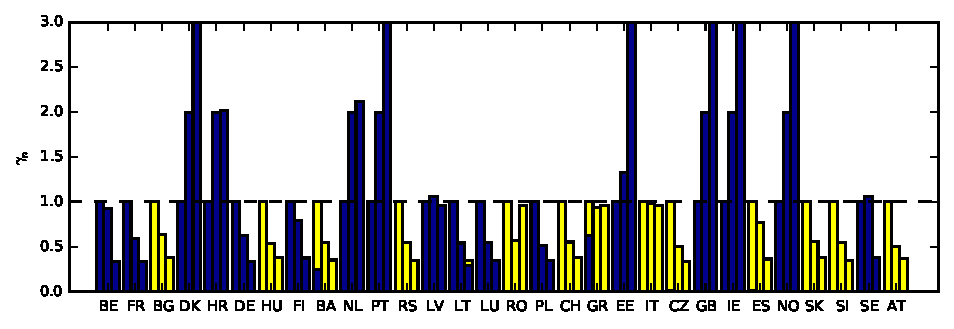
\includegraphics[width = \chromowidth, center]{gasLayouts}
    \caption{GAS optimized layouts.}
    \label{fig:agdOpt}    
  \end{subfigure}
  \caption{Optimal layouts. In each sub figure, three sets of bars
    corresponding to values of K = 1 (left), 2 (middle), and 3 (right)
    are shown.}
  \label{fig:optLayouts}
\end{figure*}

 % \begin{figure*}[p]
 %   \centering
 %   \begin{subfigure}{2\columnwidth}
 %     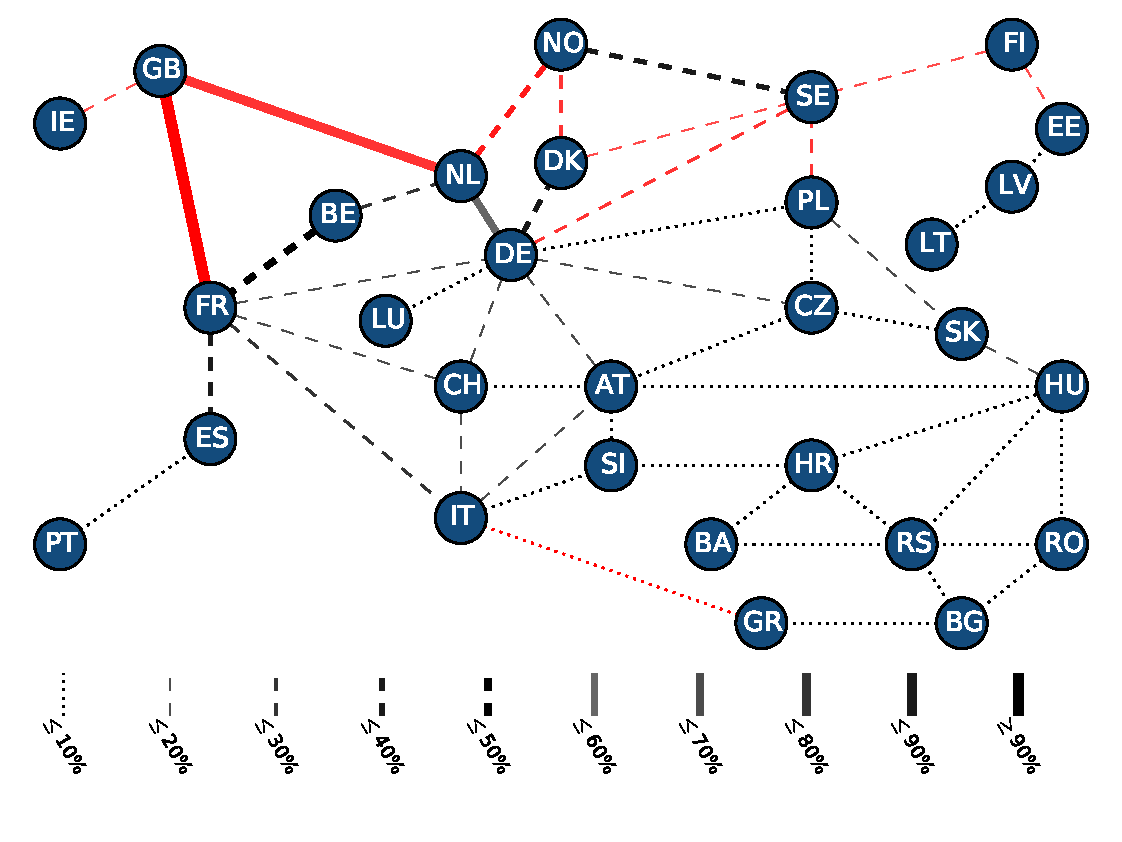
\includegraphics[width = 0.75 \columnwidth, center]{cfMaxK=3LINKS}
 %     \caption{Link usage for the CF layout constrained by K = 3.}
 %     \label{fig:linksCfMax}    
 %   \end{subfigure}
 %   \begin{subfigure}{2\columnwidth}
 %     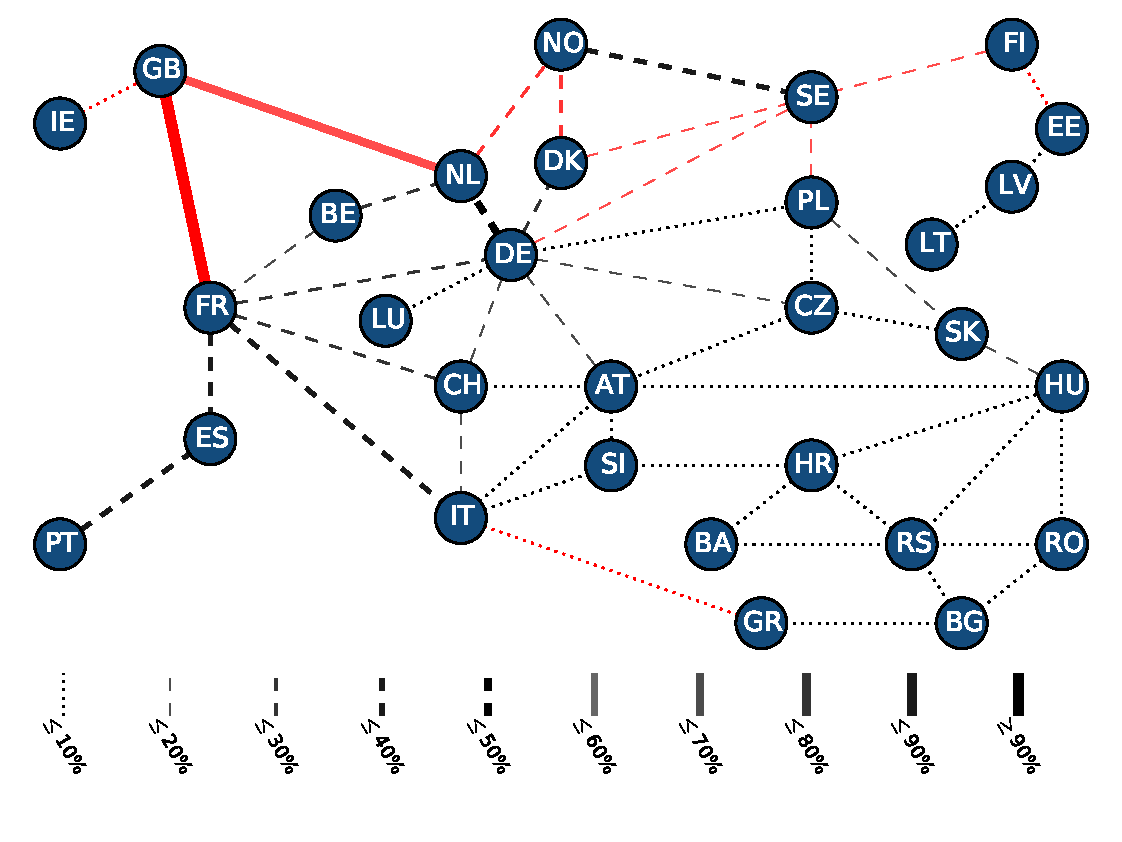
\includegraphics[width = 0.75 \columnwidth, center]{seqK=3localizedLINKS}
 %     \caption{Link usage for the GAS layout constrained by K = 3.}
 %     \label{fig:linksTransAgd}    
 %   \end{subfigure}
 %   \caption{Overview of link usage. AC links are shown in black while
 %     HVDC links are shown in red. Link capacities are indicated
 %     relative to the highest flow (110 GW between Great Britain and
 %     France in \cref{fig:linksCfMax}). In the GAS layout, resources
 %     are allocated in a way that tends to decrease the load on
 %     especially the HVDC links. This tendency can be attributed to the
 %     fact that the cost of HVDC links is significantly higher than the
 %     cost of AC links. An exception is Great Britain where $\nu^{W}$ is
 %     so high that the resulting low cost of wind energy outweighs the
 %     cost of the HVDC connections.}
 %   \label{fig:links}
 % \end{figure*}

\section{Sensitivity analysis}
\label{sec:sensitivity-analysis}

%\subsection{Excluding transmission in the optimization}
%\label{sec:incl-transm-optim}
%
%While the main findings include only three optimized layouts, for K =
%1, 2 and 3, numerous optimizations must be performed to allow
%convergence analysis, parameter tuning, and sensitivity analysis. In
%this case, each optimization taking more than a day is impractical. 
%
%As mentioned in \cref{sec:cuckoo-search}, the computation time can be
%decreased by analysing only a subset of the 32 years of data. However,
%going below one year is not ideal as this choice would imply
%neglecting important seasonal fluctuations. Numerically, the most
%costly operation in the analysis is the quadratic optimization problem,
%\cref{eq:step1}, which is solved in each iteration to determine the
%flows. This step is not needed to determine backup properties. By
%skipping the step, it is possible to speed up the optimization by more
%than a factor of 50. Layouts obtained by optimization excluding
%transmission are shown in \cref{fig:cost-no-transmission}.
%
%\begin{figure}[h!]
%  \centering
%  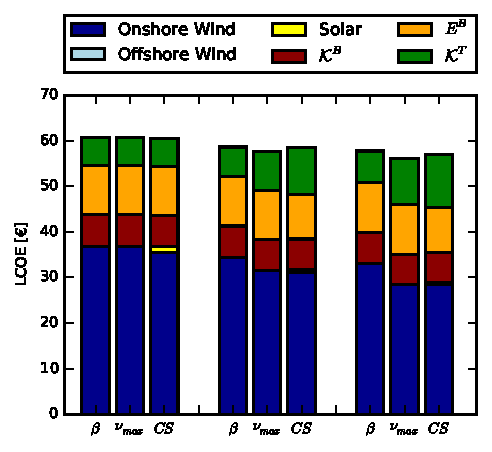
\includegraphics[width = \columnwidth]{costTransVE50}
%  \caption{Cost details for the optimal layouts for K = 1 (left), 2
%    (middle) and 3 (right) for $\beta$, CF and CS (transmission excluded).}
%  \label{fig:cost-no-transmission}
%\end{figure}
%
%It is clear that the optimization succeeds in decreasing the cost of
%all, but the transmission component. However, for K = 2 and K = 3, the
%associated increase in transmission cost is so large that the CS
%layouts end up being more expensive than the CF layouts at
%$\alpha = 1$. The difference between the CS layouts with transmission
%included/excluded is noticeable, but the CS solution obtained without
%transmission is still fairly good. For convergence analysis, parameter
%tuning, and sensitivity analysis, optimizations have been performed
%excluding transmission costs. This includes all CS solutions presented
%in this section.
%
%To illustrate how the CS solution changes when transmission is taken
%into account, the link usage for the two solutions for K = 2 is shown
%in \cref{fig:links}.
%
%\begin{figure*}[p]
%  \centering
%  \begin{subfigure}{2\columnwidth}
%    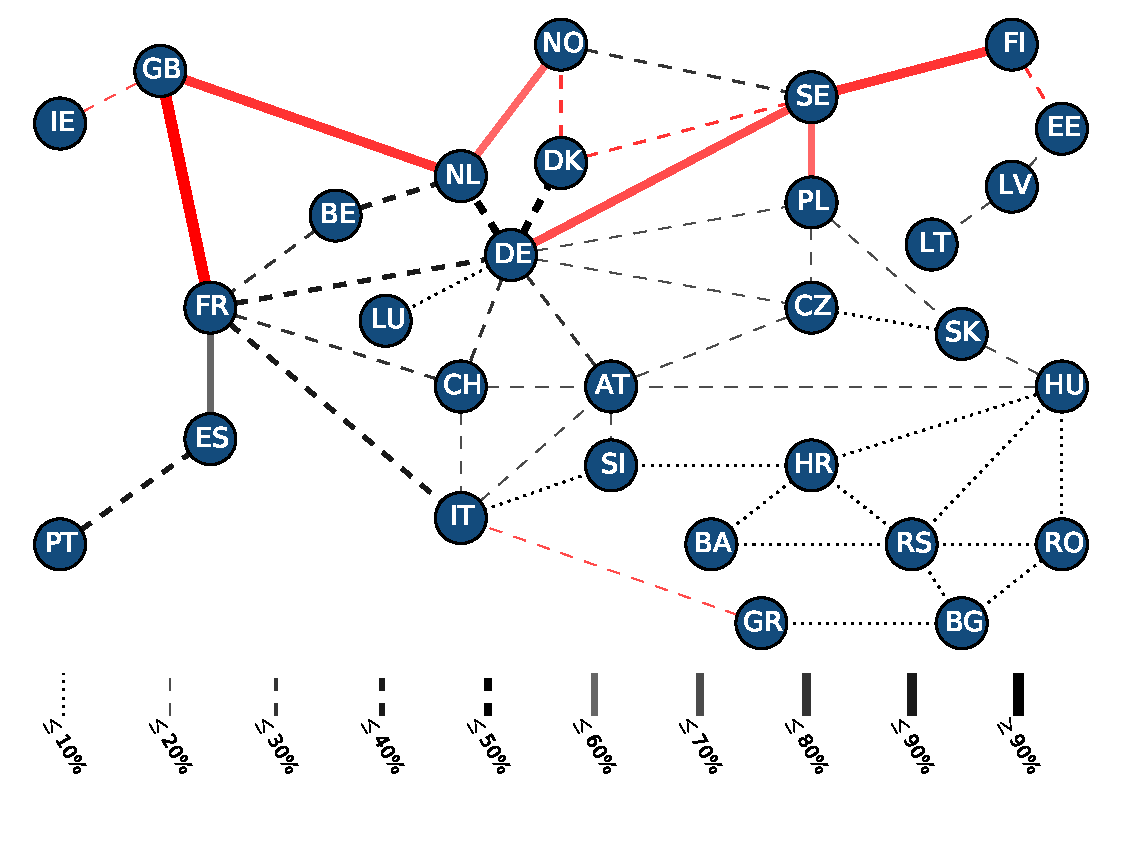
\includegraphics[width = 0.75 \columnwidth, center]{VE50cuckooK=2@defaultLINKS}
%    \caption{Link usage for the CS layout (transmission excluded)
%      constrained by K = 2.}
%    \label{fig:linksNoTrans}    
%  \end{subfigure}
%  \begin{subfigure}{2\columnwidth}
%    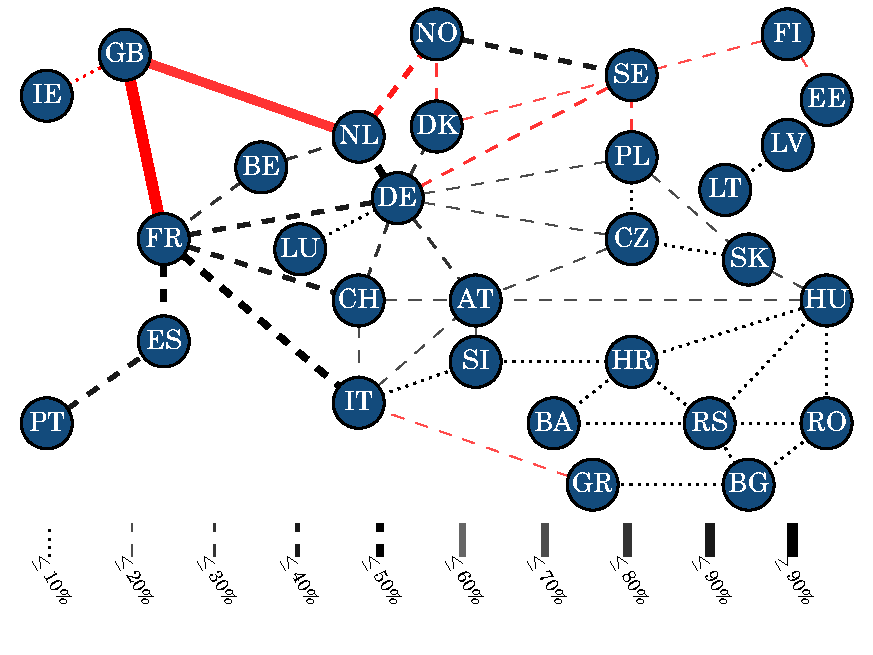
\includegraphics[width = 0.75 \columnwidth, center]{VE50cuckooK=2@TRANS10kLINKS}
%    \caption{Link usage for the CS layout (transmission included)
%      constrained by K = 2.}
%    \label{fig:linksTrans}    
%  \end{subfigure}
%  \caption{Overview of link usage. AC links are shown in black while
%    HVDC links are shown in red. Link capacities are indicated
%    relative to the highest flow (74 GW between Great Britain and
%    France in \cref{fig:linksNoTrans}). As transmission costs are included in
%    the optimization, the layout is altered in a way that tends to
%    decrease the load on HVDC links. This tendency can be attributed
%    to the fact that the cost of HVDC links is significantly higher
%    than the cost of AC links. An exception is Great Britain where
%    $\nu^{W}$ is so high that the resulting low cost of wind energy
%    outweighs the cost of the HVDC connections.}
%  \label{fig:links}
%\end{figure*}
%
%From \cref{fig:links} we see that in the CS layout obtained with
%transmission included, the resources have been reallocated in such a
%way that the link usage is decreased. In particular, the load on HVDC
%links (shown in red) is lower. Since the cost of HVDC links is
%significantly higher than the cost of AC links, it makes perfect sense
%that the load on these links has been decreased the most.

\subsection{Reduced solar cost}
\label{sec:reduced-solar-cost}

For the $\beta$ as well as the CF layouts, the optimal $\alpha$ values are
0.84. As mentioned previously, wind domination is partly a consequence
of the higher cost of energy production for solar PV compared to
onshore wind. The cost of solar has dropped rapidly in the recent
years and this tendency might very well continue. To shred some light
on the consequences of further price reductions, the sensitivity of
the optimal mix to reductions in the solar cost is examined. In
\cref{fi g:red-solar}, the LCOE as a function of $\alpha$ is shown (similar
to the lower left of \cref{fig:overview}) when the solar cost is
reduced by 25\%, 50\% and 75\% respectively.

\begin{figure*}[p]
  \centering
  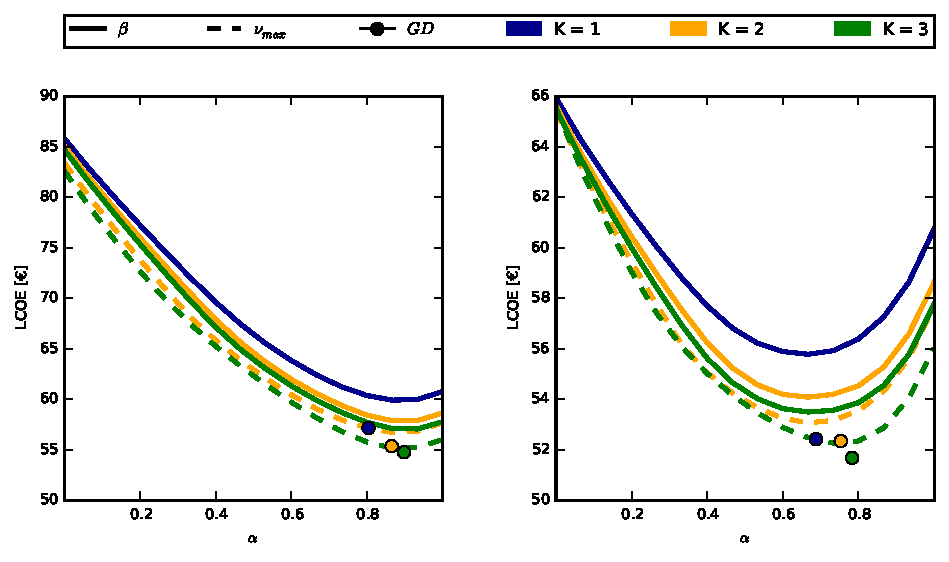
\includegraphics[width = 2\columnwidth]{solarAnalysis}
  \caption{LCOE for different magnitudes of the solar cost
    reduction. Shown are cost reductions by 0\% (top left), 25\% (top
    right), 50\% (bottom left) and 75\% (bottom right). The 0\%
    scenario serves as the reference scenario.}
  \label{fig:red-solar}
\end{figure*}

A reduction of the solar cost by 25\% does not change the picture
much. The optimal mix is shifted from above 0.8 to below 0.8 and the
cost drops slightly. As the solar cost is reduced by 50\% the cost of
pure solar ($\alpha=0$) becomes comparable to the cost of pure wind
($\alpha=1$). The optimal mix drops to around 0.6 and the LCOE is reduced
by 4.80 \euro{}
compared to the reference scenario (GAS layouts at K = 3). Reducing
the cost of solar by 75\% changes the curve shapes completely as solar
is now much cheaper than wind. With values in the 0.2 to 0.6 range,
the optimal mix now depends strongly on the choice of layout
strategy. An additional significant drop in cost is observed and for
the GAS optimized layouts at K = 3 the 50 EUR barrier is breached.

% The
%exact optimal mix $\alpha$ values are listed in \cref{tab:solar-alpha}.

% DROP VALUES: 1.82 at 25\%, 4.80 at 50\%, 9.09 at 75\% (comared to
% reference scennario, GAS optimised layouts at K = 3.

% \begin{table}[h!]
%   \centering
%   \caption{Alpha values for optimal layouts for different scalings of
%     the solar cost.}
%   \label{tab:solar-alpha}
%   \begin{subtable}{\columnwidth}
%     \centering
%     \caption{Cost reductions by a factor of 2.} 
%     \begin{tabular}[h!]{l c c c}\toprule
%       & K = 1 & K = 2 & K = 3 \\ \midrule
%       $\beta$ & 0.87 & 0.87 & 0.93 \\ 
%       CF & 0.87 & 0.87 & 0.87 \\ 
%       GAS & 0.80 & 0.87 & 0.90 \\ \bottomrule
%     \end{tabular}
%     \vspace{10pt}
%   \end{subtable}
%   \begin{subtable}{\columnwidth}
%     \centering
%     \caption{Cost reductions by a factor of 4.} 
%   \begin{tabular}[h!]{l c c c}\toprule
%     & K = 1 & K = 2 & K = 3 \\ \midrule
%     $\beta$ & 0.67 & 0.67 & 0.67 \\ 
%     CF & 0.67 & 0.67 & 0.73 \\ 
%     GAS & 0.69 & 0.75 & 0.78 \\ \bottomrule
%   \end{tabular}
% \end{subtable}
% \end{table}

\subsection{Offshore wind}
\label{sec:offshore-wind}

So far, wind has been assumed to be onshore only. By January 2014, the
total European onshore wind capacity was 120.8GW, while the offshore
capacity was 8.0GW \cite{EWEA}. While these numbers confirm the onshore
only assumption to be reasonable, the increasing share of offshore
wind raises the question, how the LCOE will be affected by the
introduction of an offshore component. The immediate expectation would
be a significant increase in the LCOE since the cost of offshore wind
is more than 100\% higher compared to onshore wind due to foundation
expenses and increased maintenance costs. On the other hand the
capacity factors for offshore sites are generally higher than for
onshore sites - but nowhere near 100\%.

It would be possible to introduce offshore wind on equal footing with
onshore wind and solar PV. However, since offshore wind is much more
expensive, an optimized layout would pose a 0\% offshore component,
which is not an interesting nor surprising result. Instead, a fixed
offshore component is introduced by splitting the wind component into
an onshore $\gamma^{W}$ and an offshore $\gamma^{\tilde{W}}$ component,

\begin{equation}
  \label{eq:11}
  \gamma^{W} = \gamma^{\text{W}} + \gamma^{\text{$\tilde{W}$}}, 
\end{equation}

for countries with suitable offshore regions. Explicitly these are:
Denmark, Germany, Great Britain, Ireland, the Netherlands, France,
Belgium, Norway and Sweden. Other countries retain onshore wind
only. The magnitude of the offshore component is defined by requiring
that the offshore wind power generation accounts for a fixed share of
the total wind power generation,

\begin{equation}
  \label{eq:12}
  \text{offshore share = }\frac{\gamma^{\tilde{W}}}{\gamma^{W}}.
\end{equation}

Cost details for optimized layouts with fixed offshore shares of 0\%, 25\% and
50\% are shown in \cref{fig:cost-offshore}.

\begin{figure}[h!]
  \centering
  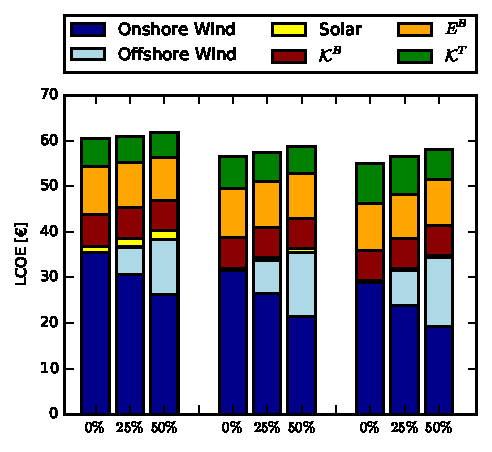
\includegraphics[width = \columnwidth]{costOffshoreVE50}
  \caption{Cost details for the GAS optimal layouts for K = 1 (left),
    2 (middle) and 3 (right) for offshore shares of 0\%, 25\% and 50\%.}
  \label{fig:cost-offshore}
\end{figure}

From \cref{fig:cost-offshore} it is clear that the introduction of an
offshore component increases the LCOE. However, the increase in LCOE
is not dramatic. While the cost of wind energy increases
significantly, the cost of backup and transmission decreases
slightly. The decrease is a consequence of the difference in the
temporal production pattern from onshore to offshore wind. In some
time steps the onshore production is low while the offshore production
is high. The introduction of an offshore component thus tends to
smooth out the wind production time series. %As a side effect, opposite
%of what one might have expected, solar becomes less favourable as
%illustrated by \cref{fig:cost-offshore}. 
The GAS optimized layouts for
an offshore share of 50\% are shown in \cref{fig:layout-offshore}.

\begin{figure*}[t!]
  \centering
  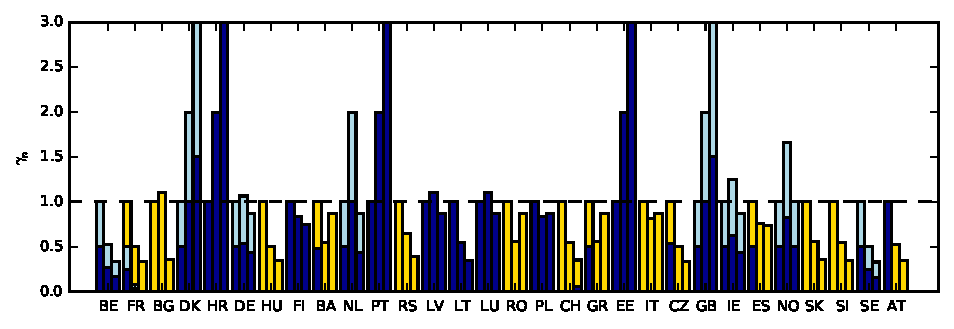
\includegraphics[width = 2\columnwidth, center]{offshoreLayouts}
  \caption{GAS layouts constrained by K = 1 (left), 2 (middle) and 3
    (right) for an offshore share of 50\% for Denmark, Germany, Great
    Britain, Ireland, the Netherlands, France, Belgium, Norway and
    Sweden.}
  \label{fig:layout-offshore}
\end{figure*}

%*************************************************************************
\section{Discussion and conclusions}
\label{sec:four}
%*************************************************************************

The dependence on the countrywise layout of VRES of a number of key
parameters along with the resulting LCOE has been investigated. It was
found that the backup and transmission costs are significant, but the main
costs are associated with the VRES capacities. The VRES capacity costs
can be lowered by allocating more resources to countries with high
capacity factors. At a heterogeneity factor of $K = 2$, meaning that
each country installs VRES capacities covering a minimum of 50\% and
maximum of 200\% of their mean load, the LCOE can be lowered by almost

% REWRITE THIS PART

5\% by choosing the heuristic CF layout which maximises the
overall capacity factor. Further reduction of the cost can be achieved
by reducing backup and/or transmission costs. Using a gradient descent
routine, a such layout was found to reduce the LCOE by an additional
2\%. While the additional cost reduction of 2\% relies heavily on the
current network structure, the primary cost reduction is of a more
general nature. 

It can be attributed to the general tendency for the
heterogeneous layouts to shift wind capacities towards the North Sea
countries. Since the wind resource quality is better than for the
central and southern countries, the reallocation results in lower
costs.

% REWRITE THIS PART

Comments on reduced solar cost ...

% A cost reduction of 7\% compared to the homogeneously might seem
% minor, but since the cost of a ?? is on the ??? scale, 7\% is
% actually a very significant cost reduction.

%The cost reduction is a strong argument for a heterogeneous
%layout. However, the realisation might be a political challenge. Since
%the optimal placing of resources was derived from a system
%perspective, a realisation would require full collaboration from all
%countries. Countries with low capacity factors would no longer be self
%sufficient, and they would be forced to invest in foreign
%capacities. Convincing countries to let go of the independence of
%their electricity system and to move capital abroad might require some
%political effort. On the other hand, locating sufficient sites for
%onshore wind in the North Sea countries might very well pose a
%challenge too.

% The cost optimal layouts considered in the main analysis are almost
% exclusively based on onshore wind. The reason is that onshore wind is
% significantly cheaper than solar, partly due to lower capital
% expenses, partly due to higher capacity factor. It was found that the
% cost of solar must decrease by a factor of $\approx$ 2 for a
% significant solar component to become profitable. Besides lowering the
% capital expenses, the solar cost could also be lowered by increasing
% the capacity factor. Based on data from \cite{REA}, the capacity factor can
% be increased by $\approx$ 40\% by applying dual axis tracking compared
% to the fixed position installation assumed in
% \cref{tab:capacity-factors}. In addition, studies on increasing the
% energy conversion efficiency are still being conducted.

The main analysis considered onshore wind only, but the effect of
introducing an offshore component was also discussed. Foundation
expenses and increased maintenance costs makes offshore wind
significantly more expensive than onshore wind. Some of the additional
expenses are compensated by higher offshore capacity factors along
with a more stable temporal production pattern, but at the end of the
day, offshore wind is still more expensive than onshore wind. However,
there are other incentives for offshore wind. The opposition from
residents is usually lower than for onshore wind, and the potential
for expansion larger. The number of suitable onshore sites are final,
and when they are exhausted, offshore wind might pose the best
alternative.

% REWRITE THIS PART 

In conclusion, it was found that a heterogeneous layout with wind
resources shifted towards the North Sea countries decreases the LCOE
by around 5\% compared to the homogeneous layout at the optimal mix. An
additional reduction by 2\% was possible by taking also transmission
and backup costs into account. \newline

The effect of integrating one or more storage elements in the
electricity system has not been considered in this paper. Promising
storage projects are already in the making, so by the time Europe reaches
$\gamma = 1$, commercial large scale storage systems are presumably
available. A natural extension of this paper would be to include
various types of storage.

%Even moderate amounts of
%storage can decrease the backup needs significantly[REF].

%For small amounts of storage, the optimal mix will most likely be
%lowered, as the day-night cycle solar makes it

% An exploration of layouts of VRES capacities over Europe shows that
% heterogeneous layouts are capable of significantly increasing the
% overall capacity factor $\nu_\text{EU}$ of renewables, while reducing
% the standard deviation $\sigma_\text{EU}$ of their generation. By scaling
% the regional penetration of renewables according to countries'
% capacity factors, we produce a heterogeneous mixture that favours
% installation primarily in countries around the North Sea, since wind
% is preferable to solar to increase $\nu_\text{EU}$ and reduce
% $\sigma_\text{EU}$. These improvements lead to an overall reduction in
% the cost of electricity generated by the system.

% Optimal layout theory helps analyse the space of heterogeneous
% layouts. By mixing wind- and solar-only layouts that lie along the
% Pareto front, we find configurations that further reduce the risk
% ($\sigma_\text{EU}$) while increasing the return
% ($\nu_\text{EU}$). However, the increased heterogeneity that these
% systems propose imply such an increase in transmission that the
% total system cost is greater than a system scaling by regional
% capacity factors. A genetic algorithm is the used to further explore
% heterogeneous layouts. With the explicit aim of reducing system
% costs, the genetic algorithm finds a very heterogeneous system that
% is nonetheless able to significantly reduce system costs, mainly
% through a marked increase in the European capacity factor
% $\nu_\text{EU}$.

% nu is defined by country-wide avetage, thats why spainis os bad,
% ahigher reoltuon might show interesting results

%\FloatBarrier

% *************************************************
\section*{Bibliography}
% *************************************************

\bibliographystyle{unsrt}%model3-num-names}
\bibliography{references}

% \clearpage
% \appendix

% %\subsection{Cuckoo search}
% %\label{sec:cuckoo-search}
% %
% % A European VRES layout is determined by the vectors
% % $\boldsymbol \gamma$ and $\boldsymbol \alpha$, each with dimensionality
% % $n$ equal to the number of nodes. For notational convenience, a
% % complete solution vector $\boldsymbol x$ is constructed as
% % $x_{1} = \gamma_{1}, ..., x_{n} = \gamma_{n}, x_{n+1} = \alpha_{1}, ...,
% % x_{2n} = \alpha_{n}$.
% % The entries of the solution vector must fulfil the constraints

% % \begin{align}
% %   \frac{1}{K} &\leq \gamma_{i} \leq K, \label{eq:kLimits}  \\
% %   0 &\leq \alpha_{i} \leq 1, \label{eq:aLimits} \\
% %   \sum_{i} \gamma_{i} \langle L_{i} \rangle &= \langle L_{EU} \rangle
% %   . \label{eq:yLimits}
% % \end{align}

% For notational convenience, a complete layout vector $\boldsymbol x$
% is constructed as
% $x_{1} = \gamma_{1}, ..., x_{N} =\gamma_{N}, x_{N+1} = \alpha_{1}, ...,
% x_{2N} = \alpha_{N}$.
% The optimization objective is global minimization of the LCOE as a
% function of $\boldsymbol x$. The LCOE is a complicated function of the
% layout $\boldsymbol x$ for which derivative information is not
% available. With 30 countries, the dimensionality of the problem is 60,
% and the search space thus large.

% Efficient global optimization within a large search space is a problem
% which has been successfully addressed by a number of Nature inspired
% meta heuristic algorithms. By imitating the best features in nature,
% these algorithms achieve a unique balance between intensification
% (search around the current best
% solution\footnote{In this section, the terms \textit{layout} and
%   \textit{solution} are used interchangeably.})
% and diversification (exploration of the search space). Typical
% examples are genetic algorithms \cite{Goldberg1989} and particle swarm
% optimization \cite{Kennedy95}. In this paper, a recent addition
% \cite{YangDeb} to the family, cuckoo search (CS), has been applied.

% %Cuckoo birds practice an aggressive breeding behaviour where the female
% %cuckoos lay their eggs in the nests of other birds. If the host bird
% %discovers the alien egg, the egg is thrown away, or the nest is
% %abandoned. To avoid this fate, some cuckoo species have specialized in
% %mimicking the visual appearance of the egg of the host species
% %cite{Payne2005}. 
% In the CS algorithm, the cuckoo eggs represent solutions. The nest is
% simply a container holding one or more eggs. For simplicity, each nest
% will hold only one egg. The actual implementation differs slightly
% across the literature\cite{YangDeb,Walton,Tuba}, but most
% implementations follow a common structure:

% \begin{enumerate}
% \item Initially, each of the $X$
%   nests are populated by an egg selected randomly from within the
%   solution space.
% \item A fraction $p$ of the eggs are discovered by the host bird and
%   abandoned.
% \item New eggs are generated and dropped into the nests. The receiving
%   nest rejects the worse of the two eggs.
% \item Step 2 and 3 are repeated until a user defined termination
%   criteria is fulfilled.
% \end{enumerate}

% %Inspired by the flight pattern of fruit flies\cite{Reynolds}, new eggs
% New eggs are generated by Lévy flights. A Lévy flight is a random walk with the
% Markov property. The step size is drawn from a Lévy
% $\alpha$-stable distribution%\footnote{The original author and
%   %others\cite{YangDeb,Walton,Tuba} use a symmetric Lévy distribution
%   %($\beta = 0$). However, it was found that the algorithmic performance,
%   %at least for the problem at hand, was increased significantly by
%   %changing to an asymmetric distribution.}
% with scale parameter $c = 1$, location parameter $\mu = 0$, stability
% parameter $\alpha = 1/2$ and skewness parameter $\beta = 1$. The large tail
% causes occasional jumps ensuring efficient diversification. The Lévy
% distribution was generated using a general method for generation of
% Lévy $\alpha$-stable distributions\cite{Weron1994}.

% % The Lévy flight was simulated using Mantegna's
% % algorithm\cite{Mantegna}.

% % In a Lévy flight, the
% % following state $\boldsymbol x (t+1)$ depends only on the current
% % state $\boldsymbol x(t)$,

% % \begin{equation}
% %   \boldsymbol x (t+1) = \boldsymbol x(t) + \alpha \mbox{Lévy}(\lambda)
% % \end{equation}

% % where $\alpha$ is a problem dependent scaling parameter. A Lévy flight is a
% % random walk with the step size drawn from the heavy-tailed Lévy
% % distribution

% % \begin{equation}
% %   \label{eq:3}
% %   \mbox{Lévy}(\lambda) \sim u = t^{-\lambda}, \mbox{ } (1 < \lambda \leq 3) 
% % \end{equation}

% % which has infinite variance and infinite mean. The large tails causes
% % occasional jumps and thus ensures efficient exploration of the
% % solution space.

% \begin{algorithm*}[t]
%   \caption{Pseudo code for the cuckoo search implementation. The
%     \textit{Evaluate} function evaluates egg costs. By passing an
%     array of eggs to the \textit{Evaluate} function, rather than
%     evaluation the eggs one by one, parallel evaluation is
%     possible. The \textit{Sort} function sorts the eggs by cost in
%     ascending order.}
%   \label{csAlgo}
%   \begin{algorithmic}
%     \Function{CuckooSearch}{}
%     \State \textit{nests} $\gets$ $X$ eggs selected randomly from within the
%     solution space
%     \State Evaluate(\textit{nests})
%     \State Sort(\textit{nests})
%     \State \textit{bestNest} $\gets$ \textit{nests[0]}
%     \State \textit{generation} $\gets$ 0
%     \While{termination criteria not fulfilled}
%     \For{index \textit{i} of bad nests} 
%     \State \textit{nests[i]}$\gets$ levy flight starting from \textit{nests[i]}
%     \EndFor
%     \For{index \textit{i} of good nests} 
%     \State \textit{trailEggs[i]}$\gets$ levy flight starting from \textit{nests[i]}
%     % \State \textit{j} $\gets$ index of a random good nest
%     % \If{\textit{i} == \textit{j}}
%     % \State \textit{trailEggs[i]} $\gets$ levy flight starting from \textit{nests[i]} 
%     % \Else   
%     % \State \textit{trailEggs[i]} $\gets$ interpolation between
%     % \textit{nests[i]} and \textit{nests[j]}  
%     % \EndIf
%     \EndFor
%     \State Evaluate(\textit{nests})
%     \State Evaluate(\textit{trailEggs})
%     \For{index \textit{i} of trailEggs} 
%     \State \textit{j} $\gets$ index of a random nest
%     \If {cost of \textit{nest[j]} $>$ cost of \textit{trailEggs[i]}}
%     \State \textit{nest[j]} $\gets$ \textit{trailEggs[i]}
%     \EndIf
%     \EndFor
%     \State Sort(\textit{nests})
%     \State \textit{bestNest} $\gets$ \textit{nests[0]}
%     \State \textit{generation} $\gets$ \textit{generation} + 1
%     \EndWhile
%     \State \Return \textit{bestNest}
%     \EndFunction
%   \end{algorithmic}
% \end{algorithm*}

% % The only major
% % difference is fixation of the scaling parameter $\alpha$ which was found to
% % improve performance significantly.

% In the CS implementation used in this paper, the nests are split into
% \textit{bad nests} (the to-be-abandoned $p$ fraction) and
% \textit{good nests} (the remaining $1-p$ fraction). The eggs in the
% bad nests are replaced immediately by new ones generated by Lévy
% flights starting from the old eggs. New trail eggs are generated by
% Lévy flights starting from the eggs in the good nests. Each trail egg
% is dropped into a random nest, and the receiving nest rejects the
% worse of the two eggs. A value of $p$ around $0.75$ gave the best
% performance. Mimicking of the host egg, approximated by the current
% best egg $\boldsymbol x_{best}$, is modelled by biasing the Lévy
% flight towards $\boldsymbol x_{best}$. In practice, the step size is
% scaled by a factor of
% $\paren{\boldsymbol x_{best}- \boldsymbol x_{i}}$. The Lévy flight
% thus takes the form

% \begin{equation}
%   \label{eq:1}
%   \boldsymbol x \to \boldsymbol x + A \paren{\boldsymbol x_{best}- \boldsymbol x} \mbox{Lévy}(z) 
% \end{equation}

% where $A$ denotes a problem specific scaling parameter. For most
% problems (the current included), a value $A \approx 1$ is appropriate. It is
% possible that a solution generated by Lévy flight is outside the
% search space defined by \cref{eq:k-factor} and the implicit constraint
% $0 \leq \alpha_{n} \leq 1$. In this case, any invalid value is shifted to
% the nearest boundary value. %: A value of $\alpha_{n} = 1.1$ is changed to
% %$\alpha_{n} = 1.0$ while a value of $\gamma_{n} = \frac{1}{K+2}$ is changed to
% %$\gamma_{n} = \frac{1}{K}$.

% % The interpolation was performed as a simple linear interpolation
% % between two solutions $\boldsymbol x_{i}$ and $\boldsymbol x_{j}$
% % 
% % \begin{equation}
% %   \label{eq:1}
% %   \boldsymbol (\boldsymbol x_{i},\boldsymbol x_{j}) \to \boldsymbol x_{i} +
% %   B \paren{\boldsymbol x_{j}- \boldsymbol x_{i}} 
% % \end{equation}
% % 
% % where $\boldsymbol x_{i}$ denotes the better of the two solutions. In
% % accordance with \cite{Walton}, $B$ was fixed at the golden ratio. The
% % interpolated solution is thus closer to the better of the two
% % solutions. 

% When a solution is generated, the solution is renormalized by a linear
% scaling of the $\gamma$ values such that

% \begin{equation}
%   \label{eq:10}
%   \sum_{n} \gamma_{n} \langle L_{n} \rangle = \langle L_{EU} \rangle
% \end{equation}

% is fulfilled. If the renormalized solution violates
% \cref{eq:k-factor}, it is rejected and a new one generated. This
% procedure is repeated until a valid solution is found.

% The termination criteria was chosen as a fixed number of
% iterations. In each iteration, $X$ function evaluations are performed,
% each requiring a loop through the 32 year dataset solving a quadratic
% optimization problem at each time step. Therefore, a single function
% evaluation takes around 15 minutes on a standard laptop anno 2015. To
% decrease computation time, a single model year was used rather than
% the full 32 year data set.

% Starting from a completely random population, it was found that around
% 50,000 function evaluations were required to reach a stable
% solution%\footnote{Non-biased optimizations and parameter tuning were
%   %performed excluding transmission costs to decrease computation time,
%   %see \cref{sec:incl-transm-optim} for details.}.
% It is possible to decrease the required number of function evaluations
% by planting a best-guess solution in the initial population. The
% drawback of this approach is the biasing of the search. Other,
% potentially better, solutions are less likely to be found due to the
% initial biasing. Starting from random populations, the stable points
% obtained for K = 1, 2, 3 were all found to be very similar to the
% CF solutions. This indicates that the CF solution is
% probably close to the global optimum. Therefore, the final
% optimizations have been performed biased by the CF solution
% effectively decreasing the number of required function evaluations by
% almost an order of magnitude. With these approximations, the
% computation time is decreased from $\approx$ 1.5 years to less than
% two days.

% For the problem at hand, the performance of the CS algorithm turned
% out to be relatively insensitive to changes in $A$, $p$ and
% $X$. Values of $A$ between 1 and 50 resulted in similar performance,
% while larger values of $A$ caused a drop in performance, probably due
% to the average step size becoming too large. Likewise, values of $p$
% between 0.65 and 0.85 resulted in similar performance, while values
% outside this interval caused drops in performance. For $X$, the best
% performance was observed around a value of 50. Values below 25 and
% above 100 caused the algorithm to get stuck in local minima.

% In building a layout where locations with high capacity factors were
% preferred to locations with low ones, one could have expected a
% larger reduction in the need for backup energy and power
% ($E^B$,\,$\mathcal K^B$). However, correlations between resources
% can either contribute or detract to the overall performance of a
% layout. A single place can have a high capacity factor, but carry a
% large risk in the form of standard deviation. This is a well known
% problem in finance, where a layout of investments must be chosen
% so as to maximise the returns while minimising risk. In this case,
% returns can be seen as a layout-wide capacity factor, $\nu_\rm{EU}$
%\begin{equation}
% \nu_\rm{EU} = \sum_n \nu_n^W \frac{\gamma_n^W \mean{L_n}}{\mean{L_\rm{EU}}} + \sum_n \nu_n^S %\frac{\gamma_n^S \mean{L_n}}{\mean{L_\rm{EU}}}
%\end{equation}
%while the risk can be related to the layout-wide standard deviation,
% as defined in (\ref{eq:stdev}). A geographical dispersion of VRES
% capacities can help reduce the total standard deviation, as wind is
% generally uncorrelated beyond 500 km.  Figure 5.2 is a
% representation of the layout of wind capacities in Europe. Each
% of the gray dots represents a randomly assigned set of wind
% capacities $\bs \gamma^W$. The homogeneous layout can be seen near the
% centre of the cloud, with a low risk but a low return (capacity
% factor). As the layout begins to favour locations with a higher
% $\nu_n^W$ via the factor $\beta$, the return of the system increases,
% without a large decrease in the risk of the investment. Layout
% theory allows us to define a Pareto front of optimal layouts,
% where we must choose between a lower risk and a higher return. This
% front is sketched via the squares in Figure 5.2.  A similar set of
% Pareto-optimal layouts can be found for the solar resources. The
% optimal wind capacities $\bs \gamma^W$ coming from Figure 5.2 can be
% combined with the optimal solar capacities $\bs \gamma^S$ via the mixing
% parameter $\alpha$. Figure 5.3 shows these interpolations, redrawing the
% homogeneous and proportional layouts we have previously discussed
% and adding several interpolations of new layouts coming from
% layout theory. We choose one of these interpolations as a
% \textbf{ Pareto-optimal layout}. The lines connecting these points
% run from $\alpha = 0$ in the solar-only layout (bottom right) to
% $\alpha = 1$ in the wind-only layout (top right). It is clear that
% moving from a pure-solar to pure-wind only increases the capacity
% factor, but there seems to be a minimum risk point close to
% $\alpha = 1$. This hints at a synergy between wind and solar resources,
% reinforcing the results in Figure 5.1 of an optimal value of $\alpha$.

\end{document}